%%%% CS 383 HW #4 - hw4-jank6275.tex
%%%% Due on BBLearn before 10pm on Friday 3/4/2016


%###############################################################################
% Header
%###############################################################################

\documentclass[11pt]{report}

\usepackage{graphicx}
\usepackage{caption}

\marginparwidth 0.5in 
\oddsidemargin 0.25in 
\evensidemargin 0.25in 
\marginparsep 0.25in
\topmargin 0.0in 
\textwidth 6in \textheight 8.5in

\title{Squire: A Collaborative Software Development Tool}
\author{Brandon Jank (jank6275@vandals.uidaho.edu)}

\begin{document}

\maketitle

\tableofcontents



%###############################################################################
% Overview
%###############################################################################
\chapter{Overview and Scope}
    \begin{minipage}{1\textwidth}
        \begin{center}
            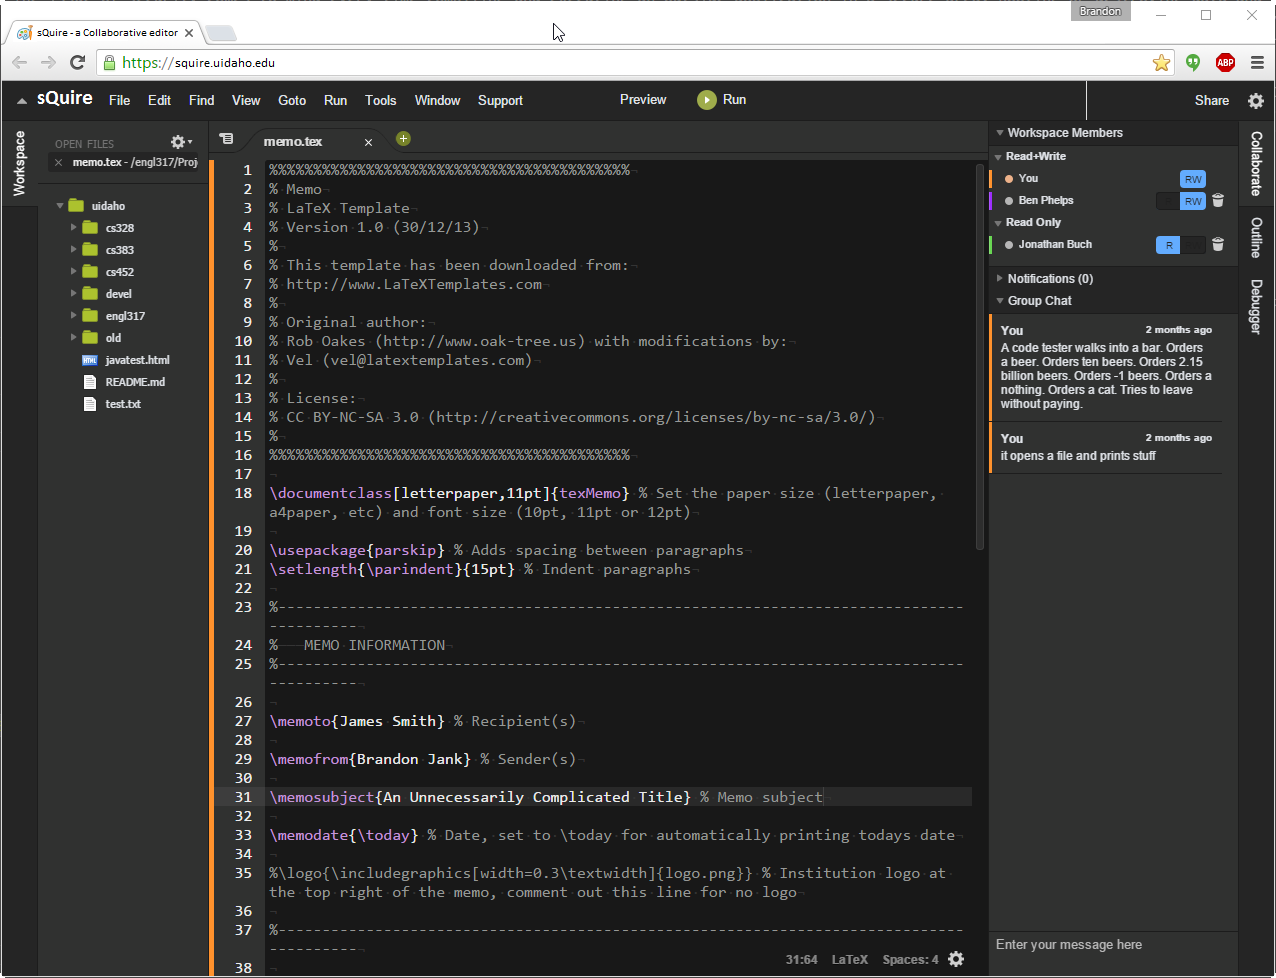
\includegraphics[width=0.7\textwidth]{squire}
        \end{center}
        \captionof{figure}{"Squire is a web-based collaborative software development environment with a project development center. Squire will allow multiple users to edit files and communicate in real time. Projects can be ``stubbed'' out by a user and then other users can join and/or vote to support for their favorite projects. After a certain amount of support, planning, and documentation is reached for a project, the project becomes a fully fleged project and then community development can start. Think ``kickstarter for code'' where people pledge their help with the project and not just financial support."}
    \end{minipage}

\section{Core Features}
    \begin{itemize}
      \item Web based
      \item Some Common IDE features
      \item Collaborative tools
      \item Encapsulated Workspaces
      \item Compile and Download
      \item Self Destructing Rooms
    \end{itemize}
    The central idea behind sQuire is a somewhat akin to a code hostel. A collaborative editor which provides private, but shareable on demand spaces, with a low overhead for creation and ease of use. These spaces are meant for short term use, over an indeterminate period. Once the collaboration is done, the space is cleared and made available for others to use.
    
    With this vision in mind, sQuire best accomodates its users by being a browser based application. There should be no need for a user to download a client program, which would require periodic updates and ultimately require deletion on the users' end. By doing all of the collaboration and storage on a central server, accessed by the browser, we can make it more accessible to a wider audience. It may also encourage the development of collaborative ``toy'' projects by making it easier to start project spaces and find assistance when a project stalls.
    
    sQuire will be focused on coding in the Java language, though there are many worthwhile languages to choose from. Focusing on a single language will allow us to add more IDE-like features to assist in collaboration and make the language more accessible to those learning it.
    IDE-like Features:
    \begin{itemize}
      \item Key word color coding
      \item Parenthesis mismatch detection
      \item Missing end of line detection/prompting
    \end{itemize}
    
    sQuire is a collaborative tool, rather than a fully featured IDE with step through run-time debugging. Its features should be geared towards making it easier to debug code collaboratively, in the browser, without over-reliance on other tools. At a minimum, it needs:
    \begin{itemize}
      \item Native chat functionality
      \item Author attribution for code (colored underlining, footnote, etc.)
      \item Ability to jump to another user's cursor
      \item Ability to import/export code as plain text
      \item Account based access to projects
    \end{itemize}
    
    Collaborative features that would be nice:
    \begin{itemize}
      \item Ability to save and restore to snapshots of the project
      \item Achievement and statistic tracking
    \end{itemize}
    
    User workspaces will be encapsulated, for both security and privacy. This could be accomplished using a container solution such as Docker or lmctfy (a free Google version). Containers have a lower performance hit to the host server than virtual machines, which are also a commonly implemented solution.  
    
    While security is a concern, we hope to address this using user space encapsulation, and by not running user code on the server. When users compile code, the compiled jar is downloaded and run locally from their own machines. While this means users are responsible for vetting the function of the code before running it on their machines, it means that our server resources are not being used as part of a bot net or similar exploit.
    
    Finally rooms must be self-destructing. For the convenience of the user, deletion of the space should be automatic after an appropriate period of inactivity. While a notification email should be sent to the space owner prior to deletion, again no user intervention should be required.

\section{Security Nightmare}
    The issue of security comes to mind every time compiling and executing an outside application in a secure area. Rooting or destroying data and infrastructure is trivial when you are freely allowed to execute arbitrary Java. In order to allow for this functionality we must implement some type of security strategy. We could limit or block functionality in Java which is a cat and mouse game that breaks usability. We could compile and execute code on the client side. Using a web browser, this would require a compiler written in JavaScript and cause compatibility issues on certain clients with reduced permissions or an exotic build environment. Or we could just Docker.


    Docker allows us to create containers that contain not only the user's build environment, but the server infrastructure to host their project. Containers include the application and all of its dependencies, but share the kernel with other containers. Simply put, users can destroy their own containers but nobody else’s. Obviously we will want to harden against known and obvious vectors, but at least any damage a user can do is limited to their own project. Containerization also allows us to take snapshots so that even if something goes wrong, we can always revert back to a working state.



%###############################################################################
% Requirements Documentation
%###############################################################################
\chapter{Requirements Documentation}
\section{Functional Requirements}
    Functional requirements will specify a behaviour or function. Squire's functional requirements are:
    \subsection{Communication (jank6275)}
        \begin{itemize}
            \item Global chat when anywhere in program. (Usecase 3.1.2 and Class 4.2)
            \item Project chat when a project is open. (Usecase 3.1.1 and Class 4.2)
            \item Closeable project chat. (Usecase 3.1.3 and Class 4.2)
            \item Closeable global chat. (Usecase 3.1.4 and Class 4.2)
        \end{itemize}

\section{Non-Functional Requirements}
    Non-functional requirements cover all the remaining requirements which are not covered by the functional requirements. They specify criteria that judge the operation of a system, rather than specific behaviours. Squire's non-functional requirements are:
    \begin{itemize}
        % Performance (jank6275)
        \item The current location of any user's cursor can be quickly jumped to by any user with the project open. (Usecase 4.5.8 and Class 5.9)
        \item Text written by the user in the editor should be visible instantaneously. (Usecase 4.5 and Class 5.9)
        \item Text written by other users in the editor should be visible within 2 seconds. (Usecase 4.5 and Class 5.9)
        \item Text will be underlined in the user's color, if they edited/created that text. (Usecase 4.5.9 and Class 5.9)
        \item The line number will be highlighted in the users color, if they created the line. (Usecase 4.5.9 and Class 5.9)
        \item Each line edited by a user should be saved to create a edit history for each user in a document. (Usecase 4.5.4 and Class 5.9)
    \end{itemize}



%###############################################################################
% Use Case Diagrams
%###############################################################################
\section{Use Case Diagrams}
    \subsection{Overview}
        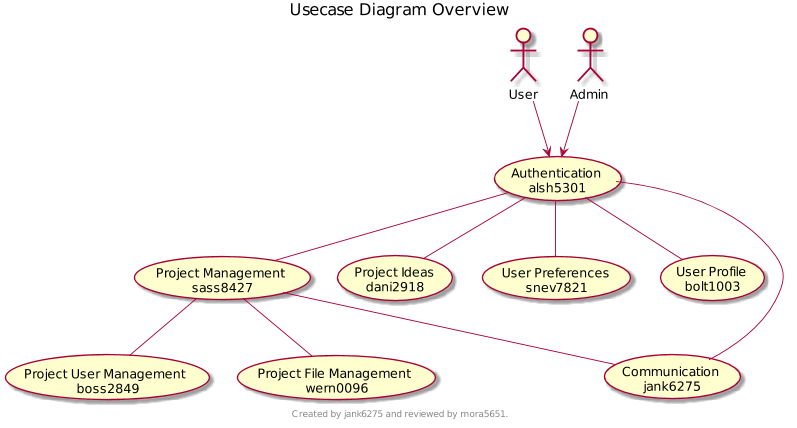
\includegraphics[width=\textwidth]{diagrams/usecase-overview}
        A usecase diagram that relates major sections of Squire.
    \subsection{Communication}
        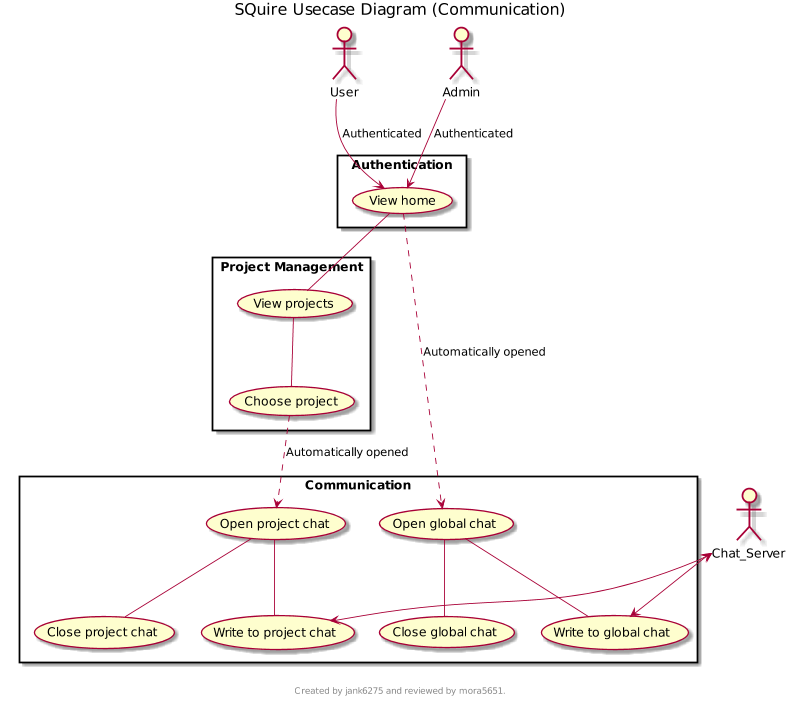
\includegraphics[width=\textwidth]{diagrams/usecase-communication}
        A usecase diagram for sQuire\'s communication features. Used in Class Diagrams 4.2.1 and 4.2.2.



%###############################################################################
% Use Case Descriptions
%###############################################################################
\chapter{Use Case Descriptions}

\section{Communication (jank6275)}
\subsection{Open project chat (Class Diagram 4.2.1)}
\begin{tabular}{ p{2cm} p{12cm} }
 \hline
 \\
 \textit{Actors:} & User \\ 
 \\
 \textit{Goals:} & To open the project chat window. \\
 \\
 \textit{Pre-conditions:} & User must be registered, signed in, and have a open project.  \\
 \\
 \textit{Summary:} & User opens a project and the project chat automatically opens. The chat window displays chat history and updates when new chat messages are received. \\ 
 \\
 \textit{Related use cases:} & Join global chat. \\ 
 \\
 \textit{Steps:} & \begin{enumerate}
  \item User opens a project.
  \item Chat is notified that user has joined.
  \item System displays project chat window to the user.
 \end{enumerate} \\
 \\
 \textit{Alternatives:} & None. \\
 \\
 \textit{Post-conditions:} & None. \\
 \\
\hline
\end{tabular}

\subsection{Open global chat (Class Diagram 4.2.1)}
\begin{tabular}{ p{2cm} p{12cm} }
 \hline
 \\
 \textit{Actors:} & User \\ 
 \\
 \textit{Goals:} & To open the global chat window. \\
 \\
 \textit{Pre-conditions:} & User must be registered, signed in, and anywhere on website.  \\
 \\
 \textit{Summary:} & User authenticates with the server and the global chat automatically opens. The chat window displays chat history and updates when new chat messages are received.  \\ 
 \\
 \textit{Related use cases:} & Join project chat. \\ 
 \\
 \textit{Steps:} & \begin{enumerate}
  \item User clicks open global chat.
  \item Chat is notified that user has joined.
  \item System displays global chat window.
 \end{enumerate} \\
 \\
 \textit{Alternatives:} & None. \\
 \\
 \textit{Post-conditions:} & None. \\
 \\
\hline
\end{tabular}

\subsection{Close project chat (Class Diagram 4.2.1)}
\begin{tabular}{ p{2cm} p{12cm} }
 \hline
 \\
 \textit{Actors:} & User \\ 
 \\
 \textit{Goals:} & To close the project chat window. \\
 \\
 \textit{Pre-conditions:} & User must be registered, signed in, and in editor Mode.  \\
 \\
 \textit{Summary:} & User clicks on close project chat and the chat window closes. \\ 
 \\
 \textit{Related use cases:} & Close global chat. \\ 
 \\
 \textit{Steps:} & \begin{enumerate}
  \item User clicks close project chat.
  \item Chat is notified that user has left.
  \item Client closes project chat window.
 \end{enumerate} \\
 \\
 \textit{Alternatives:} & None. \\
 \\
 \textit{Post-conditions:} & None. \\
 \\
\hline
\end{tabular}

\subsection{Close global chat (Class Diagram 4.2.1)}
\begin{tabular}{ p{2cm} p{12cm} }
 \hline
 \\
 \textit{Actors:} & User \\ 
 \\
 \textit{Goals:} & To close the global chat window. \\
 \\
 \textit{Pre-conditions:} & User must be registered, signed in, and anywhere on website.  \\
 \\
 \textit{Summary:} & User clicks on open global chat and the chat opens, displaying chat history and updating when needed. \\ 
 \\
 \textit{Related use cases:} & Close project chat. \\ 
 \\
 \textit{Steps:} & \begin{enumerate}
  \item User clicks close global chat.
  \item Chat is notified that user has left.
  \item Client closes global chat window.
 \end{enumerate} \\
 \\
 \textit{Alternatives:} & None. \\
 \\
 \textit{Post-conditions:} & None. \\
 \\
\hline
\end{tabular}

\subsection{Write to project chat (Class Diagram 4.2.1)}
\begin{tabular}{ p{2cm} p{12cm} }
 \hline
 \\
 \textit{Actors:} & User \\ 
 \\
 \textit{Goals:} & To send text to project chat. \\
 \\
 \textit{Pre-conditions:} & User must be registered, signed in, a project opened, with the project chat window open, and the text box selected.  \\
 \\
 \textit{Summary:} & User clicks in the project chat text box and then types a message then either presses enter or clicks the submit button. The text is displayed to all users in the chat, including the user. \\ 
 \\
 \textit{Related use cases:} & Write to global chat. \\ 
 \\
 \textit{Steps:} & \begin{enumerate}
  \item User clicks in the project chat box.
  \item User types a message and then presses enter or clicks submit button.
  \item Message is relayed to all clients with project chat open.
  \item Message is displayed.
 \end{enumerate} \\
 \\
 \textit{Alternatives:} & None. \\
 \\
 \textit{Post-conditions:} & None. \\
 \\
\hline
\end{tabular}

\subsection{Write to global chat (Class Diagram 4.2.1)}
\begin{tabular}{ p{2cm} p{12cm} }
 \hline
 \\
 \textit{Actors:} & User \\ 
 \\
 \textit{Goals:} & To send text to global chat. \\
 \\
 \textit{Pre-conditions:} & User must be registered, signed in, anywhere on website, with the global chat window open, and the text box selected.  \\
 \\
 \textit{Summary:} & User clicks in the global chat text box and then types a message then either presses enter or clicks the submit button. The text is displayed to all users in the chat, including the user. \\ 
 \\
 \textit{Related use cases:} & Write to project chat. \\ 
 \\
 \textit{Steps:} & \begin{enumerate}
  \item User clicks in the global chat box.
  \item User types a message and then presses enter or clicks submit button.
  \item Message is relayed to all clients with global chat open.
  \item Message is displayed.
 \end{enumerate} \\
 \\
 \textit{Alternatives:} & None. \\
 \\
 \textit{Post-conditions:} & None. \\
 \\
\hline
\end{tabular}

\subsection{Modify chat font (Settings Class Diagram)}
\begin{tabular}{ p{2cm} p{12cm} }
 \hline
 \\
 \textit{Actors:} & User \\ 
 \\
 \textit{Goals:} & To change a users font style inside the global and project chat. \\
 \\
 \textit{Pre-conditions:} & User must be registered, signed in, the user settings window opened, and the chat settings tab open.  \\
 \\
 \textit{Summary:} & The user clicks the settings menu and changes their font style for both the project and global chat through a drop down box of available fonts. \\ 
 \\
 \textit{Related use cases:} & Modify chat color. \\ 
 \\
 \textit{Steps:} & \begin{enumerate}
  \item User clicks the settings menu.
  \item User clicks chat settings tab.
  \item User clicks chat font drop down box.
  \item User clicks desired font.
  \item User clicks save.
  \item The user's selection is saved in the database.
  \item All further chat messages will use the selected font.
 \end{enumerate} \\
 \\
 \textit{Alternatives:} & None. \\
 \\
 \textit{Post-conditions:} & None. \\
 \\
\hline
\end{tabular}

\subsection{Modify chat color (Settings Class Diagram)}
\begin{tabular}{ p{2cm} p{12cm} }
 \hline
 \\
 \textit{Actors:} & User \\ 
 \\
 \textit{Goals:} & To change a users font color inside the global and project chat. \\
 \\
 \textit{Pre-conditions:} & User must be registered, signed in, the user settings window opened, and the chat settings tab open.  \\
 \\
 \textit{Summary:} & The user clicks the settings menu and changes their font color for both the project and global chat through a drop down box of available colors. \\ 
 \\
 \textit{Related use cases:} & Modify chat font. \\ 
 \\
 \textit{Steps:} & \begin{enumerate}
  \item User clicks the settings menu.
  \item User clicks chat settings tab.
  \item User clicks chat color drop down box.
  \item User clicks desired color.
  \item User clicks save.
  \item The user's selection is saved in the database.
  \item All further chat messages from the user will use the selected color.
 \end{enumerate} \\
 \\
 \textit{Alternatives:} & None. \\
 \\
 \textit{Post-conditions:} & None. \\
 \\
\hline
\end{tabular}



%###############################################################################
% Class Diagrams
%###############################################################################
\chapter{Class Diagrams}
\section{Overview (brec9824, jank6275)}
    \begin{minipage}{1\textwidth}
        \begin{center}
            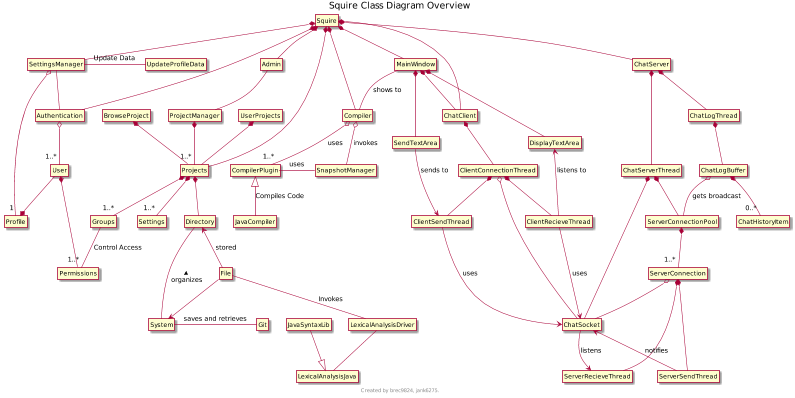
\includegraphics[width=1\textwidth]{diagrams/class-overview}
        \end{center}
        \captionof{figure}{Class overview of Squire displaying the connections between each subsystem and their classes.}
    \end{minipage}

\newpage

\section{Communication (jank6275)}
    \subsection{Client}
        \begin{minipage}{1\textwidth}
            \begin{center}
                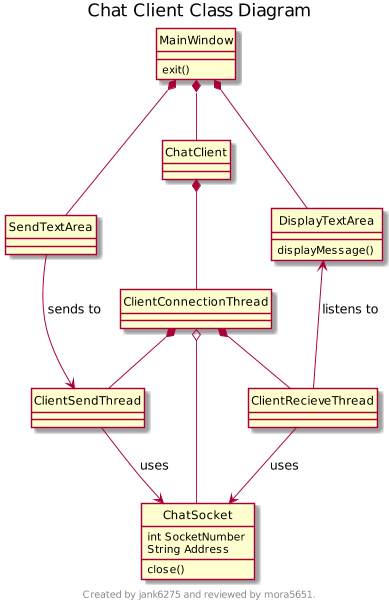
\includegraphics[width=0.7\textwidth]{diagrams/class-communication-client}
            \end{center}
            \captionof{figure}{The ChatClient class will handle text communication in conjuction with the ChatServer class. The Main Window will be home to the ChatClient. The ChatClinet will consist of client send/recieve threads to handle user input/output in the Main Window via the ChatSocket.}
        \end{minipage}
    \subsection{Server}
        \begin{minipage}{1\textwidth}
            \begin{center}
                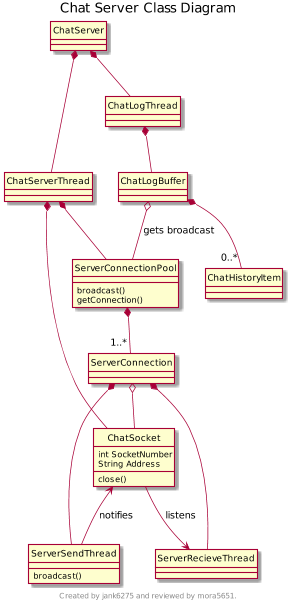
\includegraphics[width=0.5\textwidth]{diagrams/class-communication-server}
            \end{center}
            \captionof{figure}{The ChatServer class will handle text communication between ChatClient(s). The ChatLogThead records any messages broadcast by chat clients in the ServerConnectionPool as a ChatHistoryItem. Each ServerConnection consists of a send and recieve thread that utilize the ChatSocket to broadcast messages.}
        \end{minipage}



%###############################################################################
% Sequence Diagrams
%###############################################################################
\chapter{Sequence Diagrams}
\section{Authentication (jank6275)}
    \subsection{Login}
        \begin{minipage}{1\textwidth}
            \begin{center}
                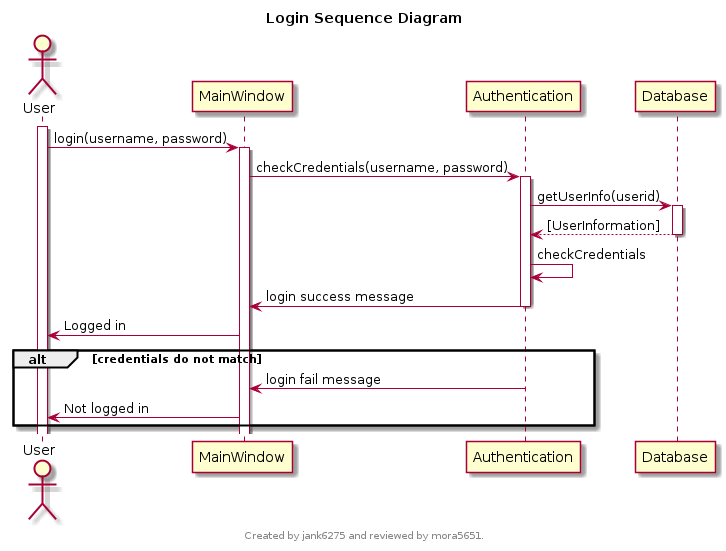
\includegraphics[width=0.7\textwidth]{diagrams/sequence-authentication-login}
            \end{center}
            \captionof{figure}{A sequence diagram for logging in to Squire.}
        \end{minipage}
    \subsection{Logout}
        \begin{minipage}{1\textwidth}
            \begin{center}
                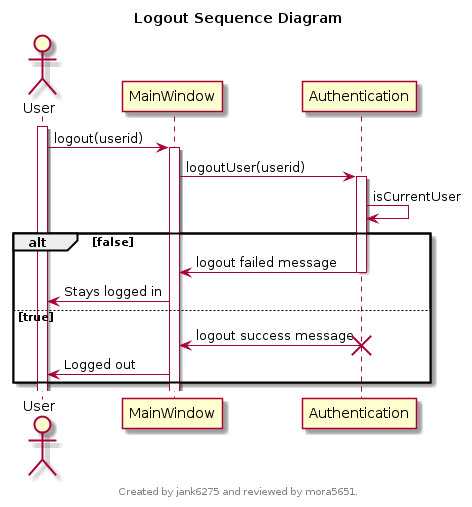
\includegraphics[width=0.7\textwidth]{diagrams/sequence-authentication-logout}
            \end{center}
            \captionof{figure}{A sequence diagram for logging out of Squire.}
        \end{minipage}
    \subsection{Register}
        \begin{minipage}{1\textwidth}
            \begin{center}
                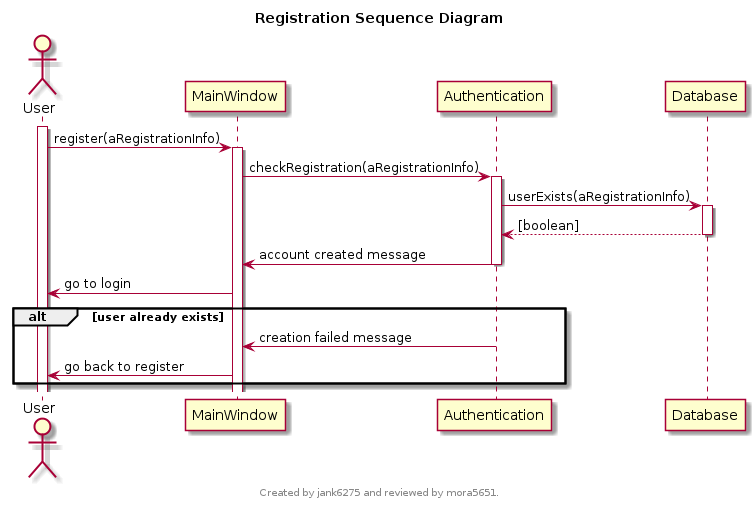
\includegraphics[width=0.7\textwidth]{diagrams/sequence-authentication-register}
            \end{center}
            \captionof{figure}{A sequence diagram for registering a nmew account with Squire.}
        \end{minipage}

\end{document}